%  LaTeX support: latex@mdpi.com 
%  For support, please attach all files needed for compiling as well as the log file, and specify your operating system, LaTeX version, and LaTeX editor.

%=================================================================
\documentclass[12pt]{article}{Definitions/mdpi} 


%=================================================================
% MDPI internal commands
\firstpage{1} 
\makeatletter 
\setcounter{page}{\@firstpage} 
\makeatother
\pubvolume{1}
\issuenum{1}
\articlenumber{0}
\pubyear{2021}
\copyrightyear{2020}
%\externaleditor{Academic Editor: Firstname Lastname} % For journal Automation, please change Academic Editor to "Communicated by"
\datereceived{} 
\dateaccepted{} 
\datepublished{} 
\hreflink{https://doi.org/} % If needed use \linebreak
%------------------------------------------------------------------


%=================================================================
% Add packages and commands here. The following packages are loaded in our class file: fontenc, inputenc, calc, indentfirst, fancyhdr, graphicx, epstopdf, lastpage, ifthen, lineno, float, amsmath, setspace, enumitem, mathpazo, booktabs, titlesec, etoolbox, tabto, xcolor, soul, multirow, microtype, tikz, totcount, changepage, paracol, attrib, upgreek, cleveref, amsthm, hyphenat, natbib, hyperref, footmisc, url, geometry, newfloat, caption

\usepackage{amssymb}
\usepackage{amsfonts}
\usepackage{amsmath}
\usepackage[nohead]{geometry}
\usepackage{pdflscape}
\usepackage[singlespacing]{setspace}
\usepackage[bottom]{footmisc}
\usepackage{indentfirst}
\usepackage{endnotes}
\usepackage{graphicx}
\usepackage{subcaption}
\usepackage{rotating}
\usepackage{threeparttable}
\usepackage{epsfig}
\usepackage{longtable} 
\usepackage{array} % for extrarowheight
\newcolumntype{H}{>{\setbox0=\hbox\bgroup}c<{\egroup}@{}}
%\usepackage{subfigure}
\usepackage{color}
\usepackage{natbib}
\usepackage{comment}
\setlength{\marginparwidth}{2cm}
\usepackage{todonotes}
\usepackage{tabularx}
\usepackage{booktabs}
\usepackage{siunitx}
\usepackage[utf8]{inputenc}
\usepackage[T1]{fontenc}
%\usepackage{lscape}

\usepackage[capitalise]{cleveref}
\graphicspath{{images/}}
\usepackage{subcaption}

\usepackage{url}

\usepackage{float}
%\usepackage[addedmarkup=uuline]{changes}

\usepackage{caption}

\usepackage{flushend}
\usepackage{graphics}
\usepackage[all]{xy}
\usepackage{tikz}

\usepackage{titling}
\thanksmarkseries{arabic}

%\usepackage{fancyhdr}
%\pagestyle{fancy}
%\fancyhf{}
\usepackage{lastpage}

%%%%%%%%

\DeclareMathOperator*{\argmax}{arg\,max}
\DeclareMathOperator*{\argmin}{arg\,min}

%%%%%%%%

\setcounter{MaxMatrixCols}{30}
\newtheorem{theorem}{Theorem}
\newtheorem{fact}{Fact}
\newtheorem{assumption}{Assumption}
\newtheorem{acknowledgement}{Acknowledgement}
\newtheorem{proposition}{Proposition}
\newtheorem{definition}{Definition}
\newtheorem{lemma}{Lemma}
\newtheorem{prediction}{Prediction}

\newenvironment{proof}[1][Proof]{\noindent\textbf{#1.} }{\ \rule{0.5em}{0.5em}}
\makeatletter
\def\@biblabel#1{\hspace*{-\labelsep}}
\makeatother
\geometry{left=1.2in,right=1.2in,top=1.2in,bottom=1.2in}


%=================================================================
%% Please use the following mathematics environments: Theorem, Lemma, Corollary, Proposition, Characterization, Property, Problem, Example, ExamplesandDefinitions, Hypothesis, Remark, Definition, Notation, Assumption
%% For proofs, please use the proof environment (the amsthm package is loaded by the MDPI class).

%=================================================================
% Full title of the paper (Capitalized)
\Title{Opening up Transactive Systems: Introducing TESS and Specification in a Field Deployment}

% MDPI internal command: Title for citation in the left column
\TitleCitation{Opening up Transactive Systems: Introducing TESS and Specification in a Field Deployment}

% Author Orchid ID: enter ID or remove command
\newcommand{\orcidauthorA}{0000-0002-6854-2653} % Add \orcidA{} behind the author's name
%\newcommand{\orcidauthorB}{0000-0000-0000-000X} % Add \orcidB{} behind the author's name

% Authors, for the paper (add full first names)
\Author{Marie-Louise Arlt$^{1,\dagger,\ddagger}$, David P. Chassin $^{1,\ddagger}${2,} and L. Lynne Kiesling $^{3}$\orcidA{}*}

% MDPI internal command: Authors, for metadata in PDF
\AuthorNames{Marie-Louise Arlt, David P. Chassin and L. Lynne Kiesling}

% MDPI internal command: Authors, for citation in the left column
\AuthorCitation{Arlt, M.; Chassin, D.; Kiesling, L.}
% If this is a Chicago style journal: Lastname, Firstname, Firstname Lastname, and Firstname Lastname.

% Affiliations / Addresses (Add [1] after \address if there is only one affiliation.)
\address{%
$^{1}$ \quad Ludwig Maximilians University Munich; marie-louise.arlt@econ.lmu.de\\
$^{2}$ \quad SLAC National Accelerator Laboratory\\
$^{3}$ \quad University of Colorado-Denver; lynne.kiesling@ucdenver.edu}

% Contact information of the corresponding author
\corres{Correspondence: lynne.kiesling@ucdenver.edu}

% Current address and/or shared authorship
\firstnote{Current address: College of Engineering, Design \& Computing, University of Colorado-Denver, Denver, Colorado 80204 USA} 
\secondnote{These authors contributed equally to this work.}
% The commands \thirdnote{} till \eighthnote{} are available for further notes

%\simplesumm{} % Simple summary

%\conference{} % An extended version of a conference paper

% Abstract (Do not insert blank lines, i.e. \\) 
\abstract{Transactive energy systems (TS) use automated device bidding to access (residential) demand flexibility and coordinate supply and demand on the distribution system level through market processes. 
In this work, we present TESS, a modularized platform for the implementation of TS, which enables the deployment of adjusted market mechanisms, economic bidding, and the potential entry of third parties. TESS thereby opens up current integrated closed-system TS, allows for the better adaptation of TS to power systems with high shares of renewable energies, and lays the foundations for a smart grid with a variety of stakeholders.
Furthermore, despite positive experiences in various pilot projects, one hurdle in introducing TS is their integration with existing tariff structures and (legal) requirements. In this paper, we therefore describe TESS as we have modified it for a field implementation within the service territory of Holy Cross Energy in Colorado. Importantly, our specification addresses challenges of implementing TS in existing electric retail systems, for instance, the design of bidding strategies when a (non-transactive) tariff system is already in place.
We conclude with a general discussion of the challenges associated with ``brownfield'' implementation of TS, such as incentive problems of baseline approaches or long-term efficiency.}

% Keywords
\keyword{electricity, transactive energy, market-based dispatch, bidding functions, automated bidding)} 

% The fields PACS, MSC, and JEL may be left empty or commented out if not applicable
%\PACS{J0101}
%\MSC{}
%\JEL{}


%%%%%%%%%%%%%%%%%%%%%%%%%%%%%%%%%%%%%%%%%%
% Only for the journal Applied Sciences:
%\featuredapplication{Authors are encouraged to provide a concise description of the specific application or a potential application of the work. This section is not mandatory.}
%%%%%%%%%%%%%%%%%%%%%%%%%%%%%%%%%%%%%%%%%%

%%%%%%%%%%%%%%%%%%%%%%%%%%%%%%%%%%%%%%%%%%
% Only for the journal Data:
%\dataset{DOI number or link to the deposited data set in cases where the data set is published or set to be published separately. If the data set is submitted and will be published as a supplement to this paper in the journal Data, this field will be filled by the editors of the journal. In this case, please make sure to submit the data set as a supplement when entering your manuscript into our manuscript editorial system.}

%\datasetlicense{license under which the data set is made available (CC0, CC-BY, CC-BY-SA, CC-BY-NC, etc.)}

%%%%%%%%%%%%%%%%%%%%%%%%%%%%%%%%%%%%%%%%%%
% Only for the journal Toxins
%\keycontribution{The breakthroughs or highlights of the manuscript. Authors can write one or two sentences to describe the most important part of the paper.}

%%%%%%%%%%%%%%%%%%%%%%%%%%%%%%%%%%%%%%%%%%
% Only for the journal Encyclopedia
%\encyclopediadef{Instead of the abstract}
%\entrylink{The Link to this entry published on the encyclopedia platform.}
%%%%%%%%%%%%%%%%%%%%%%%%%%%%%%%%%%%%%%%%%%

\begin{document}
%%%%%%%%%%%%%%%%%%%%%%%%%%%%%%%%%%%%%%%%%%

\section{Introduction}

% Motivation and contributions of this paper
Residential distribution systems are a potential source of system flexibility, particularly in demand. This potential can be realized by an approach called transactive systems (TS), which coordinates residential distributed energy resources (DER) through a market-based mechanism. 
In this work, we present Transactive Energy Service System (TESS), a modularized platform for the implementation of TS, which enables the deployment of adjusted market mechanisms, economic bidding, and the potential entry of third parties.\footnote{The code and documentation of TESS are available at \url{https://github.com/slacgismo/TESS}.} TESS thereby opens up current integrated closed-system TS, allows for the better adaptation of TS to power systems with high shares of renewable energies, and lays the foundations for a smart grid with a variety of stakeholders.
Furthermore, we describe TESS as we have modified it for a field implementation within the service territory of Holy Cross Energy, an electric cooperative serving Eagle, Pitkin, Garfield, Mesa, and Gunnison counties in Colorado. Importantly, our specification addresses challenges of implementing TS in existing electric retail systems, for instance, the design of bidding strategies when a (non-transactive) tariff system is already in place.

% Definition and brief history of TS
Transactive energy systems generally use market processes and automated device bidding to coordinate supply and demand and provide devices with control signals using price-based dispatch. The ground-breaking work in the GridWise Olympic Peninsula project demonstrated in the field that flexible devices can be controlled using a simple price-discovery mechanism to reduce energy procurement cost and manage congestion constraints to the distribution grid (see \citet{PNNL2006} and \citet{hammerstrom_2008}). Heating, Ventilation, and Air Conditioning (HVAC) systems and water heaters submitted bids for dispatch to a market operator. These bids were based on heuristic bidding functions, which resulted in higher bids for customers with higher priority.
The demand bids were settled with the available supply and resulted in a locational price for energy that equated marginal benefit and marginal cost.
This price generally equalled the marginal cost of electricity procurement if import of electricity was unconstrained, and deviated from it when transmission capacity was scarce. In the real-time market, the market design was a double auction, in which buyers and sellers submit simultaneous bids and offers, which enabled the market operator to determine a market-clearing price to push to devices. Through these mechanisms, the operators of the TS were able to reduce energy procurement cost and manage limited import capacity from the bulk power system.

% More recent work
More recent TS projects have extended this work in some economic dimensions. 
One line of work concerns device bidding.
\citet{PNNL2006} and \citet{hammerstrom_2008} initially implemented a heuristic bidding function for HVAC systems. This approach was, for instance, extended by \citet{adhikari_simulation_2016} who analyzed different approaches, with and without pre-cooling.
However, neither approach considered customers' incentives explicitly, such as the individual tradeoffs they are willing to make with regard to comfort, and how those could differ across customers with different preferences.
Instead, \citet{Arlt2020} has proposed an economically motivated bidding function for HVAC systems.
\citet{widergren_transactive_2017} further addressed this open question by describing a general framework of economic, incentive-based demand bidding.
In addition, \citet{lian_transactive_2020} have considered strategic bidding of devices, for instance under a Stackelberg model. The mentioned contributions are summarized in \cref{tab:existing_contributions_bidding}.
A second line of contributions concerns the inclusion of additional device types. While the initial pilots included HVACs, water heaters, dryers, and municipal water pumps on the demand side, with diesel and microturbine generators on the supply side, more recent work also included other DER devices.
\citet{behboodi_integration_2016} and \citet{behboodi_electric_2016} examined inclusion of electric vehicles (EVs) in TS. 
\citet{sajjadi_transactive_2016}, \citet{ableitner_user_2020}, and \citet{mengelkamp_decentralizing_2018}, among others, analyzed inclusion of photovoltaics (PV).
\citet{parandehgheibi_two-layer_2017} proposed a transactive controller for electric storage.
Third, several contributions have discussed different market mechanisms other than the central double auction. \citet{fuller_analysis_2011} and \citet{Arlt2020} analyzed the performance of double auctions in detail. \citet{widergren_residential_2014} worked with multiple feeders and transactive nodes, resulting in locational prices. Another extension has been opening up the TS architecture for peer-to-peer trading, e.g. as summarized by \citet{zhang_review_2017} and \citet{sousa_peer--peer_2019}.
Institutional concerns regarding peer-to-peer trading have, for instance, been addressed by \citet{masiello_sharing_2016}.
%Valuation: PNNL Part II \citet{lian_part_2017}, \citet{lian_transactive_2018} formulate a general valuation framework of economic bidding but do not specify their framework for any device or DER.
\citet{abrishambaf_towards_2019} provides a taxonomic survey of ongoing research efforts with regard to TS and lists relevant pilot projects in the US and in Europe. 

% Gap for TESS as a platform
The summarized literature shows that TS have been adapted continuously to reflect the new economic opportunities and challenges posed by power systems with increasing shares of renewable energy and DER.
However, opportunities remain to develop more economically-founded bidding functions and new market designs that are better able to address the new challenges of renewable energy systems with high volatility and uncertainty of generation.
In this work, we therefore introduce the Transactive Energy Service System (TESS) platform, which modularizes TS architectures in field deployment, and present its economic building blocks. 
The platform allows for continuous development of the essential components of TS.
Furthermore, the TESS design concept breaks up the closed system design that TS have usually followed in field deployment, as documented in \cref{tab:existing_contributions}. In particular, TS have been designed as a system for the utility to manage procurement cost and dispatch devices according to their priority. However, future energy systems are likely to be shaped by a variety of stakeholders offering innovative business models, including manufacturers of smart home systems and flexible devices or load aggregators. This evolution also introduces the possibility for customers to deviate from the dispatch determined by the TS instead of allowing for direct price-based control through the utility. 
Future TS must take these potential developments into account and be open for interactions that have yet to be defined. With TESS, we hope to provide a starting point for this development.

% Brownfield
Moreover, we observe that most of the implemented TS operate on the assumption that the TS fully substitutes the existing tariff system (``greenfield''). 
In that case, devices bid their marginal value (or some heuristic estimate of it) and supply is offered at marginal cost, typically the real-time wholesale market price (e.g., \citet{PNNL2006}, \citet{katipamula_transactive_2017}). Past deployments operated under experimental conditions: customers were either assigned to an experimental tariff or received side-payments for a separate billing through the TS. This context, however, does not reflect the incentive structure customers are facing in real-world implementations, with existing tariff schemes and outside options affecting the opportunity costs facing an individual customer. 

The presence of fixed retail tariffs as well as net-metering (``brownfield'') change the design requirements and conditions for TS operations. They also change customers' participation incentives by presenting them with outside options that were not available in the previous greenfield projects. 
Although a TS provides an alternative compensation mechanisms for DER that could, for example, replace net metering, existing tariff schemes or regulations are hard to change and often require approval from political bodies or regulatory commissions. 
Moreover, while some of these tariff components divert customers from efficient economic dispatch, they can serve other socioeconomic objectives or are meant to push technology adoption. It is as yet unclear how such objectives could be pursued under a TS.
Finally, power systems -- with their technical, economic, and social aspects -- are complex systems. Many of the agents involved, whether customers, utilities, or regulators, are risk-averse. 
For these reasons, the requirements of a greenfield TS have potentially hindered broad acceptance and deployment of TS in utilities across the US and explain why -- while experimental field deployments have been considered successful -- TS have not been broadly adopted in the field.
Therefore, systematic approaches for brownfield deployment might be necessary to establish the technology, learn about operational challenges, and provide the road to a true ``smart grid''.

\begin{table}[t]
\centering
\caption{Examples for operational field TS and local electricity markets}
\label{tab:existing_contributions}
\begin{tabular}{p{4cm}|p{5cm}|p{5cm}}
\textbf{Project} & \textbf{References} & \textbf{Limitations}                   \\ \hline
 Olympic Peninsula Project & \cite{PNNL2006,hammerstrom_2008} & Closed system; heuristic bidding functions; no brownfield \\ \hline
Quartierstrom & \cite{Ableitner2020,Woerner2019} & Closed system; fixed supply cost; no automated bidding determination \\ \hline
LAMP & \cite{Mengelkamp2018} & Closed system; fixed supply cost; no automated bidding determination \\
\hline
% \bottomrule
\end{tabular}
{\textit{A comprehensive review of field projects can further be found in \cite{Weinhardt2019} and \cite{abrishambaf_towards_2019}.}}
\end{table}

\begin{table}[t]
\centering
\caption{Selected contributions on TS bidding}
\label{tab:existing_contributions_bidding}
\begin{tabular}{p{5cm}|p{9cm}}
 \textbf{References} & \textbf{Limitations}                   \\ \hline
 \cite{adhikari_simulation_2016} & HVAC only; no brownfield bidding; no consistent utility framework \\ \hline \cite{Arlt2020} & HVAC only; no brownfield bidding \\ \hline \cite{behboodi_electric_2016} & EV only; heuristic bidding function; no brownfield \\ \hline
 \cite{hammerstrom_2008} & No brownfield bidding; no consistent utility framework \\ \hline
 \citet{lian_transactive_2020} & General economic framework of bidding, without specification for devices \\ \hline
 \cite{sajjadi_transactive_2016} & No active bidding, but response to real-time price signal; PV only; no brownfield bidding \\ \hline
 \cite{widergren_transactive_2017} & General economic framework of bidding, without specification for devices \\ \hline
% \bottomrule
\end{tabular}
\end{table}

In a field implementation of TESS within the service territory of Holy Cross Energy (HCE) in Colorado, we have been confronted with such brownfield conditions.
In this paper, we describe TESS as we have modified it for HCE. We focus on photovoltaics (PV) systems and elaborate how we designed bidding functions for PV given that customers usually already benefit from net metering. Under net metering, residential customers only pay for their net consumption, i.e. the value of solar generation equals the fixed retail rate, from the perspective of the customer.
This existing rate establishes an important baseline for customers' participation and bidding behavior.
We argue that, for a TS to benefit all parties, these economic incentives play a pivotal role. This claim is particularly true in brownfield deployments, where customers are already part of an existing tariff system and have outside options, such as not participating in the TS.

% Combine both contributions
By designing a TS as an open system and enabling economic bidding considering available outside options, we facilitate flexibility through mutually-beneficial exchange of electricity in the TESS design by focusing on actual \emph{price discovery} instead of generating a control signal specific to a closed system. Price discovery is the process by which producers and consumers interact to reveal not just the accounting cost of operating a supply resource, but also the actual marginal value of consumption, the opportunity costs facing both buyers and sellers, and the value of the alternatives available to them.  

We proceed as follows: In \cref{sec:background}, we summarize the history of transactive systems and the economic theory underlying our TS design. In \cref{sec:standard_design}, we describe the TESS standard design. Then, in \cref{sec:hce}, we give a description of Holy Cross Energy and the conditions of the TESS field experiment. We follow up with the modifications to our transactive system and discuss the challenges for implementation in \cref{sec:challenges}. We conclude in \cref{sec:conclusion}.

\begin{table}[ht]
\centering
%{Abbreviations\label{tab_abbr}}
%{\resizebox{\columnwidth}{!}{%
\caption{Abbreviations}
\begin{tabular}{l|l}
%\toprule

\textbf{Abbreviation} & \textbf{Description} \\
%\midrule
\hline
CPR & Critical Peak Rate \\
DER & Distributed Energy Resources \\
HCE & Holy Cross Energy \\
HVAC & Heating, Ventilation, and Air Conditioning \\
MW & Megawatt \\
MWh & Megawatt hour \\
NEM & Net Energy Metering \\
PV & Photovoltaics \\
RR & Retail Rate \\
TE & Transactive Energy \\
TESS & Transactive Energy Service System \\
TS & Transactive System
%\bottomrule
\end{tabular}
%}
%}

\end{table}

\section{Background}\label{sec:background}

The TESS platform builds on previous TS work. In this section we summarize that history (Section \ref{sec:tehistory}) and the theoretical context that is the economic foundation of our design (Section \ref{sec:teecon}).
This background provides the foundation for Section \ref{sec:standard_design} to show how TESS opens up the closed control architecture of current TS, as well as how it embodies economic theory in its emphasis on price discovery and price-based dispatch to reflect demand and DER value, opportunity costs, and outside options more explicitly in electric systems.

\subsection{Transactive Energy Background}\label{sec:tehistory} 

Transactive energy was originally conceived of as \emph{transactive control} to address the problem of integrating large numbers of small resources optimally into electric power system operations (TE 1.0).
TE 1.0 implemented the ``prices to devices'' concept by pushing a cost-based price signal to devices, observing the response, and changing the price signal iteratively to bring quantity supplied and quantity demanded into equilibrium (a process economists will recognize as Walrasian \emph{tat\^{o}nnement}). This utility-generated price signal tends to be cost-based and supply-focused, reflecting demand only to the extent that devices respond iteratively, with an objective function of achieving a particular system control objective.

Such iterative price discovery methods often introduce feedback delays that can lead to price and control instability. Hence they are not well-suited to situations where fast-acting control of DERs is desired.
Eliminating the iterative process requires large amounts of potentially private information about those resources' supply and demand functions, such as would be required for a formal numerical optimization solution. This problem has become even more prominent as utilities struggled to integrate a growing variety of behind-the-meter demand response and DERs, including photovoltaics, electrified end-uses that were previously fossil-based, electric vehicles and their chargers, and energy storage into their system operations using conventional utility programs such as energy efficiency and demand-side-management. 

The transactive energy market design developed for the GridWise Olympic Peninsula Testbed Demonstration Project \citep{hammerstrom_2008} moved beyond TE 1.0 (TE 2.0). One dimension of the project tested a real-time market, implemented as a double clock auction buyers and sellers submit bids and offers simultaneously in a specified market time interval. The market clearing provided a price signal for automated device demand response and dispatch.
Automating device participation in such markets reduces transaction costs, elicits information about relative value and relative cost from agents around the edge of the distribution network via their devices, increases the frequency of participant activity, improves responsiveness, and makes autonomous price-based dispatch feasible. 

Despite the resemblance to a market mechanism, this setup differed from an economic mechanism in several respects. First, the bids did not reflect the actual economic value customers attributed to dispatch, but rather indicated a heuristic technical prioritization. The following equation represents the bidding function of an HVAC system, the main flexible device of the Olympic Peninsular experiment:

\begin{equation}
    b_t &= p_{mean} + (T_{current} - T_{set}) \frac{k p_{var}}{|T_{lim} - T_{set}|}
\end{equation}

The bidding functions converted comfort objectives, e.g., indoor air temperature $T_{current}$, to reservation prices $b_t$ based on the expected price mean and variance. As comfort decreased, the bid price rose above the mean price $p_{mean}$, and did so more if the price variance $p_{var}$ was greater. When comfort increased the bid dropped below the mean price, and did so more if the price variance was greater. The price mean and variance were taken over the past 24 hours, which was very effective at capturing the diurnal interaction of comfort demand and price fluctuations.
Bidder priority or indication of comfort could be set through $k$. $T_{lim}$ represents the minimum or maximum price and $ T_{set}$ the respective temperature setpoint, depending on the mode of the HVAC system (heating or cooling). 
The resulting bidding function is visualized in  Figure~\ref{fig:Transactive_DA} (right).
The aggregation of individual bids gives the demand function of the system (left).

\begin{figure}[t]
\centering
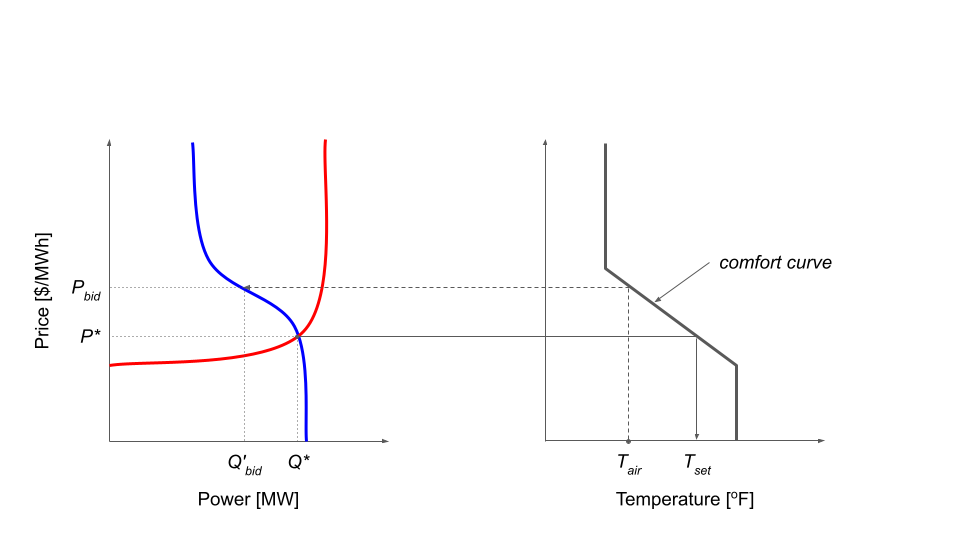
\includegraphics[scale=0.5]{images/TE_DA.png}
\caption{Transactive Double Auction (left) and Thermostat Bidding Strategy (right)}
\label{fig:Transactive_DA}
\end{figure}

However, the economic utility framework of the customers remained undefined. This heuristic approach usually creates circumstances in which devices place bids that do not reflect customers' actual marginal values and, as a result, customers might wish to deviate from a cleared bid. However, in the Olympic Peninsula project, customers could not change the TS-determined dispatch because devices were part of a closed technical control system. The only option left to customers was to override preferences (e.g., temperature setpoints) and essentially exit the TS as a flexible device for the duration of the override. In bidding functions, however, the design task is to express customers' marginal value of dispatch. Only when the bidding function reflects that marginal value do customers have no incentive to deviate from their allocation to dispatch. As a result, market clearing coincides with social welfare optimization. 

Second, because the TS was layered on top of their existing utility contract and was separate from it, customers made decisions as if no other tariff considerations interfered with their market participation (``greenfield''). Customer bidding behavior was therefore guided by the marginal cost of consumption to them (and, likewise, the marginal cost of supply for the utility). This approach ignores the complexity of outside options customers are facing, for instance because of an existing tariff system. Under a true market mechanism, customers would always consider all outside options and opportunity costs of participating in the TS.

TE 2.0, with a double auction and automated price-based dispatch, changes the paradigm to ``prices from devices'' to establish an informative market-clearing price that is then used for prioritization and dispatch. The TE 2.0 paradigm is more adaptable to unknown and changing conditions and better enables flexibility in the face of uncertainty at varying scales and time frames. It is thus well-suited to the operational challenges associated with increasing DER adoption.

\subsection{Transactive Energy Economic Theory}\label{sec:teecon}

TESS, our implementation of TE 2.0, employs a synthesis of economic market design and control systems, with an emphasis on demand-side and DER owner/operator bidding \citep{chassin2017thesis}. 
As in previous TS, it bases coordination on preference-based bids from both demand and supply agents. 
One of the most important and challenging dimensions of TS design is how the preferences of the demand-side and DER can be expressed and specified for automated bidding. 
\citet[Chapter IV]{Arlt2020} has shown how such a bidding function can be specified for HVAC systems.
Other TS models tend to fall in one of two categories: basing the device bidding on a cost-based objective, or basing the device bidding function on a technical heuristic or on an aggregate or market demand approximation \citep[Chapter IV]{Arlt2020}. Instead, TESS will enable the implementation of bidding functions that enable users to communicate their preferences for dispatch and their availability for flexible dispatch more directly.

The economic foundation of demand-side and DER bidding draws from multiple fields of economic theory \citep{kiesling_2021}. An essential feature of the economics of transactive energy is that people are distinct, with individual and private characteristics and subjective preferences over the goods and services they consume. Consumption bids should reflect their marginal willingness to pay. Producers, too, face opportunity costs that might be unknown and heterogeneous, and their perception of opportunity costs can even be subjective. Subjectivism in economic theory reflects the key insight that personal preferences and opportunity costs are private knowledge.

The preferences and opportunity costs of consumers and producers are also not knowable by or accessible to others, so coordination requires some mechanism that gives people incentives to communicate some of that subjective, private knowledge and turn it into information. That mechanism is the price system. A price system operating within a clear set of rules provides a decentralized mechanism for gathering information and learning about these preferences and opportunity costs, even among strangers (or their devices). The market process of mutual learning and decision-making enables prices to emerge that coordinate the actions and plans of all users of the system, incorporating both supply and demand information into that emergent price.

All price systems operate in an institutional framework, a set of rules, and the rules shape the incentives of participants. Effective price systems and market institutions can be challenging, or can fail to exist, due to transaction costs. When transaction costs are high and market transactions are costly to employ for coordination, other methods of organizing economic activity emerge, such as vertical integration. Technological change, most recently digitization and automation, have reduced transaction costs of using the price system relative to these other institutions \citep{kiesling_2016}. The TESS design takes advantage of these transaction cost reductions.

One institutional form for price discovery is auctions. Auctions are useful aspects of market design when the allocation problem is characterized by asymmetric information. In the case of electricity market design, the object for sale has different, subjective value to each potential bidder, a case known as a private value auction model. The double auction (DA), as discussed in Section \ref{sec:tehistory}, treats buyers and sellers symmetrically, enabling them to make simultaneous bids and offers. In a static DA, buyers submit bid schedules and sellers submit offer schedules of price and quantity \citep{friedman1993double}. The centralized auction platform performs a clearinghouse function, arranging all of the buyers’ schedules into a market demand curve and all of the sellers’ schedules into a market supply curve. 
This process enables a market price to emerge, determining quantity supplied and quantity demanded and clearing the market. 
Theoretical and experimental analysis suggests that the DA is a very efficient market design, enabling price discovery even in the presence of fragmented, private knowledge, where each participant knows only her own value/opportunity cost \citep{easley1993theories}.

Another relevant field of economics is mechanism design, a game-theoretic approach to examining situations in which individuals make decisions and interact when they have private knowledge that could affect the decisions they make and the ultimate outcomes. Mechanism design focuses on eliciting truthful revelation of some information about that private knowledge/type. Depending on the environment and the objective function of the principal, different mechanisms can perform better or worse at truthful revelation.
The general structure of mechanism design is to maximize some objective function across all $n$ individuals subject to two constraints: incentive compatibility (IC) and individual rationality or participation (IR), where $v_i$ is the value function for agent $i$, $\theta_i$ is agent $i$'s type, $g_i$ is agent $i$'s outcome, and $t_i$ is a monetary transfer to/from agent $i$.

\begin{equation}
IC: 	v_i(g^*_i(\theta_i,t_i(\hteta_i)) \geq v_i(g_i(\theta_i,t_i(\theta_i)) \qquad \forall i,g
\end{equation}

\begin{equation}
IR:	    v_i(g^*_i(\theta_i,t_i(\theta_i)) \geq 0
\end{equation}

The objective function varies depending on the specific context, but represents profit, surplus, or welfare maximization. The IC constraint ensures that each agent is better off truthfully revealing type in the outcome from the chosen mechanism compared to other alternative outcomes. The IR constraint ensures that each agent is better off participating in the system than not participating. 
Practical mechanisms that can be implemented are hard to identify, and testing such mechanisms is an essential step in overall market design. Experimental economics provides a framework for performing such market design tests, and field deployments are an example of these important tests.

These economic fields and principles inform our overall approach to market design for price discovery, and our design of device bidding functions taking into account opportunity costs and outside options to enable incentive compatible voluntary participation of agents in TESS.

\section{TESS Standard Design}\label{sec:standard_design}

In this section, we discuss which design requirements future TS need to address to integrate high levels of DER and prepare the path to a true, market-based smart grid.
We are designing the TESS platform to enable implementation of these capabilities.
Specifically, TESS design requirements include all those found in the original Olympic demonstration, as well as (1) a standardized platform that reveals the full extent of demand-side and DER flexibility, (2) economically founded bidding functions, (3) a real-time market operation capable of operating concurrently at multiple time-scales, and (4) a flexible settlement mechanism. The following sections will detail each design requirement.

\begin{figure}[!t]
    \centerline { \scalebox{0.5} { \xymatrix {
        (1)~Development
    &
    &   (2)~Deployment
    &
    &   (3)~Operations
    \\       
    &
    &   
    &
    &   *++[F]{Scheduling}
    \\      
    &   *++[F]{Financing}   \ar[r]
    &   *++[F]{Outreach}    \ar[r]
    &   *++[F]{Provision}   \ar`r[ru][ru] \ar`r[rd][rd]
    &
    \\  *++[F]{Screening}   \ar`r[ru][ru] \ar`r[rd][rd] \ar`r[rru][rru] \ar`r[rrd][rrd] \ar`r[rrru][rrru] \ar`r[rrrd][rrrd]
    &
    &
    &
    &   *++[F]{Operations}
    \\
    &   *++[F]{Engineering}      \ar[r]
    &   *++[F]{Install}     \ar[r]
    &   *++[F]{Bootstrap}   \ar`r[ru][ru] \ar`r[rd][rd]
    \\
    &   \qquad \qquad \qquad
    &
    &   \qquad \qquad \qquad
    &   *++[F]{Settlement}
    \save "1,1"."6,2"*++[F--]\frm{}\restore
    \save "1,3"."6,4"*++[F--]\frm{}\restore
    \save "1,5"."6,5"*++[F--]\frm{}\restore
    }}}
    \caption{TESS program elements}
    \label{fig:tess_program_elements}
\end{figure}

As a platform for implementing TS, the TESS modules described here are only part of a whole-of-operation approach that addresses the full life cycle of a TS deployment with an objective of integrating DER into the utility operation.  
More broadly, TESS is designed to include program development tools such as screening, financing, and engineering software, deployment tools such as participant identification, recruitment, enrollment, and bootstrapping products, as well as system operations tools such as wholesale, distribution, and settlement products to give the utility all the resources needed to successfully implement a TS.
This approach will allow different kinds of utility operations to be supported using the same system infrastructure, significantly reducing the barriers to adoption and the cost of deployment of TS. 
\cref{fig:tess_program_elements} illustrates the different program components.

\subsection{Technical Setup of Market Operations}\label{sec:technical_setup}

The code and documentation of TESS are available at \url{https://github.com/slacgismo/TESS}. The current setup reflects the specification of TESS for our field deployment in Colorado, as described in \cref{sec:hce}.

Each customer $i$ has a home hub $HH_i$ that manages the settings and actions of its devices $\mathcal{J}$ on the customer's behalf. At each market interval, the relevant physical state information $\mathcal{S}_{ijt}$ is measured by the meter or other relevant sensors and written to the TESS database on the cloud.
Based on this information, the agents representing the home hubs on the cloud update their physical states and form dispatch bids $b(\mathcal{S}_{ijt})$, i.e., how much they are willing to pay for consumption $b^d_{ijt}$ or the minimum price for supply $b^s_{ijt}$. 
The agent representing the retailer submits wholesale market supply, with the price bid $b^s_{WS}$ corresponding to the cost of supply $c^{WS}$ and the quantity bid to the import capacity. This coordination with wholesale operations is essential to ensuring that the utility is maximizing its utilization of the wholesale agreements it has in place.
Shortly before the beginning of the market interval, the market operator agent collects all bids and determines the market result by constructing market demand $D(p)$ and supply curves $S(p)$ for that interval. 

The market is cleared in a welfare-maximizing way, where quantity supplied equals quantity demanded. 

\begin{equation}
    {p_t} = & \argmax \sum_D (b^{d}_{ijt} - p_t) q^{d}_{ijt}(p_t) - \sum_S (p_t - b^{s}_{ijt}) q^{s}_{ijt}(p_t) \\ 
    &\text{s.t.} D(p_t) = S(p_t)
\end{equation}{}

The result is characterized by an equilibrium price $p_t$ and quantity $q_t = D(p_t) = S(p_t) $.
After market clearing, home hubs compare their devices' bids to the equilibrium price. If the bid price is equal to or exceeds the equilibrium price $b^d_{ijt} \geq p_t$ (for demand) or is less $b^s_{ijt} \leq p_t$ (for supply), the bid was cleared and the device is dispatched. 

All agents are implemented on the cloud and values (measurements, bids, market results) are stored in the TESS database.

Periodically the utility must settle the accumulated account balances with all the participants in the TS, as discussed in \cref{sec:settlement}.

\subsection{TESS Design: Price Discovery Mechanisms}\label{sec:price_discovery}

Price discovery occurs through the interaction of demand bids and supply offers on the market platform. 
The double clock auction mechanism is a key feature of standard TS designs. Most TS are currently designed to discover energy prices per MWh, with bid quantities in a given time period measured in MW.  The analogy to wholesale energy markets is obvious, insofar as TS are often designed to mitigate distribution constraints.
The double auction used on most existing transactive projects, however, has important limitations that TESS seeks to overcome in its design. 

First, double auctions are unable to clear resources optimally that can act significantly faster than the auction interval, or are less flexible. The typical market interval is 5 minutes, which is also implemented in TESS as a default. However, TESS allows an operator-specified market clearing interval.

Second, it is also difficult, if not impossible, to reveal any forward knowledge through the real-time double auction  mechanism, which precludes agents from making mutually beneficial forward commitments. To address these problems, as a first step, the TESS design includes an order book mechanism that accepts two types of bids: market orders and limit orders. A market order allows a resource to dispatch immediately at the current price, whatever it is. A limit order allows a resource to reveal its dispatch capabilities for any future time interval, contingent on a suitable ask or offer price. 
In a second step, forward markets should be implemented which enable resources to participate in day-ahead markets, for instance. This will be an important component to invest into flexible resources such as storage.

Third, as more DERs enter the resource mix, particularly zero marginal cost resources, changing market design away from energy as the traded good may be useful. Three different resource attributes and their prices are mathematically related: energy prices (\$/MWh), storage prices (\$/MWh$^2$), and ramping prices (\$/MW) \citep{chassin2017thesis}. TESS' modular structure is designed to support these three distinct price discovery mechanisms simultaneously. 

Ultimately, TESS will also provide multi-level market integration, from retail to feeder to wholesale.

\subsection{TESS Design: Participating Devices and Bidding Functions}\label{sec:devices}

In the standard design piloted by the Olympic project, thermostat heating/cooling devices, diesel generators, micro-turbines, white goods appliances, and municipal water pumping systems were the principal resources that could place bids and offers in the retail market.  At the time, these were the typical devices utilities hoped to dispatch using a retail real-time energy price. 
TESS enables a wide variety of resources to participate in the market, with custom bidding functions that can communicate both the technical capabilities of the resource and the preferences and opportunity costs of the owner.
More recently, new types of flexible DERs figure prominently in utility distribution system operations, so TESS also supports photovoltaics, electric vehicle chargers, and electric energy storage.

The bidding strategies devices used in the Olympic Peninsula project were selected by the system engineers, and not by the vendors or users of the devices. Given the lack of experience with TS this design choice was necessary to ensure that the system functioned properly. 
Such a design meant that the bids submitted potentially do not reflect the actual marginal value of dispatch, raising potential issues with incentive compatibility if consumers were given the capability of deviating from their bid after the market has been cleared \citep{lian_transactive_2020}. 
The high degree of automation not only ensured strong demand response resource participation, but also protected against strategic bidding practices that could undermine the design objectives of the mechanism.
Nevertheless, the system designers recognized that ultimately the bidding strategies are the most important part of the system and the design, and selection of these strategies was a task ideally left to the device manufacturers and consumers in a decentralized system.

The TESS design brings this notion to full realization by allowing device manufacturers and third-party agent developers to implement their own bidding strategies, allowing devices to have customized bidding functions and giving consumers more direct control over the settings that govern those strategies. For example, consumers can control their battery storage resource strategy by changing the preferred energy reserve (given their preference for resilience) and its sensitivity to price fluctuations (given their risk aversion). Similarly, electric vehicles can be configured to charge more aggressively, ignoring prices fluctuations, or more economically by charging only when the price is low (\cite{behboodi_electric_2016}). 

Bid function heterogeneity is another important and distinctive feature of TESS that improves price stability, and is likely to make it more difficult for one type of device or vendor to exercise any kind of market power.
The TESS design also anticipates the emergence of AI bidding agents, where learning and forecasting functionalities are included. This development is expected to bring additional diversity in the bidding strategies and add to the overall resilience and stability of the TS by avoiding many adverse ``flocking'' behaviors and resulting price volatility observed in the previously demonstrated TS.

Finally, if the market design is adjusted as described in \cref{sec:price_discovery}, bidding strategies need to be adjusted to incorporate the new set of rules.
In the case of order books, there is also a time dimension that must be included, and absent a price, the bid is considered simply a market order and the price of the next available resource is taken.

\subsection{TESS Design: Settlement Mechanisms}\label{sec:settlement}

While demand and supply coordinate in real time through a TS, the accounting to reconcile financial flows with transactions often takes place later (e.g., monthly). Several financial settlement systems have been demonstrated in previous TS, including a side-payment mechanism \citep{hammerstrom_2008} and a regulator-approved tariff \citep{Widergren2014}. 

TESS completes the settlement process in two steps. First, all the transactions since the last settlement are totaled for each participant. The utility then computes the total costs and revenues of TESS operations, to determine the net benefit of operating TESS during the settlement period.  A suitably chosen portion of total net benefit, e.g., 50\%, is then divided among all the participant \textit{pro rata} their net transactions for the period.  For example, if Alice earned \$100 during the period, and Betty earned \$50, then if the utility saw a net benefit of \$30, the payment to Alice would be \$110, and the payment to Betty would be \$55, and keep the remaining \$15. Note that this net benefit may be negative number, in which case it would reduce the participant payments in a similar manner. In addition, some participants may have negative payments, i.e., costs, in which case the credit may be offset those debits. 

In addition, TESS proposes a token-based settlement systems which also permits the use of new digital or crypto-currencies, if desired.
For instance, a certain number of tokens could be issued each month by the utility based on the expected value of the total welfare surplus from operations. Customers then participate in the transactive system using these tokens, so their token balances reflect their decisions and actions. At the end of the month the total surplus is calculated and used to assign a value to the tokens. Each participant is then compensated according to how many tokens they hold and their individual bill credits awarded accordingly. This approach uses cooperative game theory concepts about dividing a co-created benefit, and develops an indirect approach to performing a Shapley value calculation to implement that allocation.

The token-based approach has multiple advantages. 
First, the utility is not committed to compensating consumers more than the total net benefit arising from their collective behavior. In particular, if consumers exhibit a short-term behavior that is highly profitable to them but has a longer-term negative system impact, this will be revealed in reduced token values and diminish the strength of the near-term incentives relative to the long-term benefits.  
Second, the calculation methods ensure that all parties are compensated fairly for their marginal contributions to the total net benefit, i.e., a consumer whose actions increased the total surplus greater will see a larger reward than one whose actions were detrimental. Actions that are both individually and collectively beneficial are rewarded the most, and ones harmful to both are rewarded the least, while those that only benefit one or the other are rewarded somewhere in between.  
Finally, the use of tokens might open up new opportunities. For instance, customers could receive tokens for other activities which are beneficial for the system, such as sharing data or for certain energy efficiency investments.
A discussion of the challenges of working with tokens can be found in \cref{sec:impl_challenges}.


\section{The Holy Cross Energy Project}\label{sec:hce}

The initial TESS deployment and field experiment is taking place in partnership with Holy Cross Energy (HCE). The HCE implementation represent a so-called minimum viable product (MVP), and focuses only on new kinds transactive resources, i.e., photovoltaics, batteries, and electric vehicles.  Although supported by TESS, less emphasis is being placed on demand response resources like heat pumps and water heaters.  
In the following section, we describe the setting of Holy Cross Energy and their motivation to deploy a TS (\cref{sec:HCE_description}), the Basalt Vista project (\cref{sec:Basalt}), and their existing tariff structure (\cref{sec:HCE_tariff}). 

\subsection{Holy Cross Energy}\label{sec:HCE_description}

Holy Cross Energy (HCE) is a member-owned electric cooperative in Colorado. Its service territory includes the Roaring Fork Valley from Aspen to Glenwood Springs, and the Eagle River and Colorado River Valleys from Parachute to Vail, as seen in \cref{fig:HCE_service_territory}. It provides power to over 57,000 premises and operates around 3,000 miles of transmission and distribution lines, with a summer peak of 150 MW. HCE's members are predominantly residential, small commercial, and ski resorts. 

\begin{figure}[t]
\centering
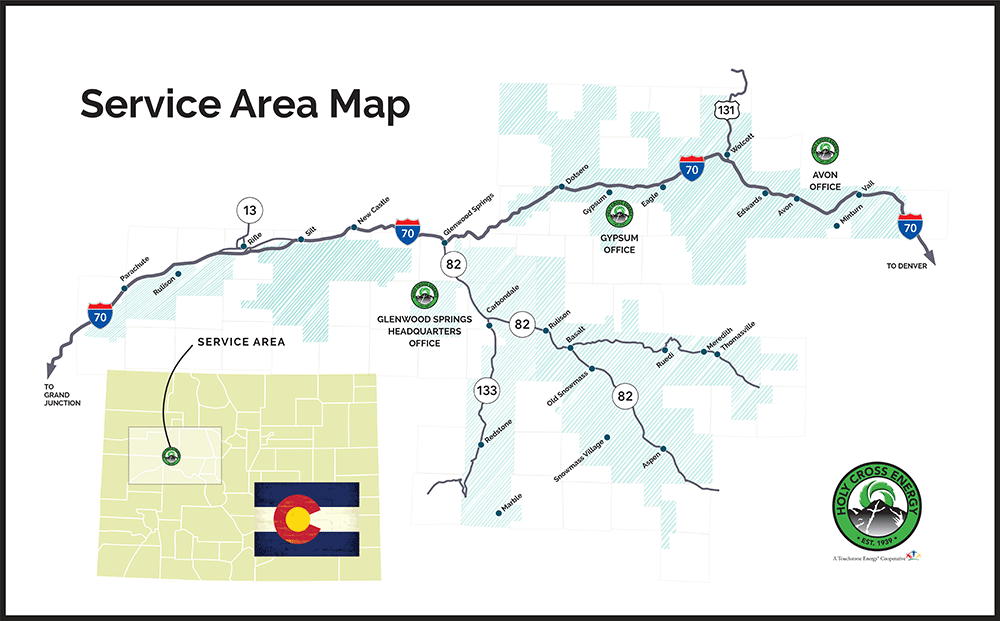
\includegraphics[scale=0.4]{HolyCrossEnergy-Service-Area-Map.png}
\caption{HCE Service Territory}
\label{fig:HCE_service_territory}
\end{figure}

HCE's load during peak periods is dominated by winter resort activity, i.e., residential and lodging loads, along with day-time winter sports and night-time snow making.  The residential and lodging loads are not sufficiently flexible to participate greatly in demand response (DR) programs. However, HCE has put in place a number of DR programs that resorts participate in should load-shedding be required, particularly for those relating to night-time snow-making demand.

HCE purchases most power on long-term contracts with Public Service Company of Colorado (an Xcel Energy company) and the Western Area Power Association. The price of electricity under the long-term contract is \$0.02/kWh but increases to \$13/kW during the monthly coincident peak, i.e. the peak of the Xcel service territory. HCE's annual peaks usually occur in late December and early January during the holiday season. The 2018 summer peak was 156.3 MW and the winter peak was 256.3 MW.  In 2018 net generation was 461 GWh and wholesale procurement was 774 GWh with retail sales of 1,233 GWh.

Furthermore, HCE is considering participating in the Western Electric Coordinating Council (WECC) energy balancing market, as part of a broader agreement between Xcel and the Western EIM operated by CAISO \citep{CAISO2020}. Under this agreement, HCE would be exposed to real-time wholesale market prices at which it could buy or sell electricity. Increased demand flexibility would enable HCE to manage its load, revenue, and costs more actively.

With regard to emissions, in 2019 HCE's fuel mix was 44 percent renewable, 40 percent coal, and 7 percent natural gas, and the remainder is unknown \citep{HCE2019}. The renewable resources are mainly wind (31 percent), biomass (7 percent), and hydro (3 percent), with the remainder solar and mine methane. HCE has an ambitious carbon reduction target of having a greenhouse gas emission-free fuel mix by 2030. In 2018 HCE set a target of 70 percent greenhouse gas emission-free by 2030, and subsequent improvements in clean energy technologies have led them to revise the target to 100 percent by 2030. To meet this goal, HCE is investing in infrastructure to increase its adoption of technologies like electric vehicles, rooftop solar PV, and storage, as well as digitization to interconnect DERs and optimize their dispatch. 

Resilience is another priority for HCE, particularly against wildfire risk. In 2018, the Lake Christine wildfire spread in the Roaring Fork Valley, causing the evacuation of thousands in Carbondale, El Jebel, Basalt, and Fryingpan Valley, and destroying over 12,000 acres. In a mountainous region with abundant large wildlife and a single transmission line, HCE faces considerable technical challenges in achieving a resilient high-DER system. Increasing DER adoption and digital interconnection will provide flexibility that contributes to resilience, and the coordination using price-based dispatch through TESS enables that flexibility.

\subsection{Basalt Vista}\label{sec:Basalt}

To learn more about DER management and to experiment with involving customers in sustainable system management, HCE and other community partners are collaborating with Habitat for Humanity to construct affordable housing in Basalt and equip it with digital and DER-enabling infrastructure. Each of the 27 houses will have solar PV, EV charging, and hookups for battery storage. The houses in the community are connected to each other and capable of autonomous energy sharing using the National Renewable Energy Laboratory's Network Optimized Distributed Energy Systems (NODES) algorithm \citep{IEEESpectrumNREL}. 

TESS is part of the larger Basalt Vista project, a collaboration between the Roaring Fork School District, which donated the land, Pitkin County, which funded the road and utilities, and Habitat for Humanity, which raised the funds to cover the gap between the costs to build the homes and the revenue from the purchase prices, as well as facilitating mortgage access and assistance.  The Community Office for Resource Efficiency helped fund the high-performance heating and photovoltaic systems. Holy Cross Energy donated the inverters, electric vehicle chargers, hot water heaters, controllers, and the batteries for the first four homes.  Additional financial support and discounts were provided by the vendors, including Bryant Colorado, Sunsense Solar, the Town of Basalt, LE, and a number of private donors. The TESS team was invited to deploy controllers in the first four houses with the goal of implementing a full Type 2.0 TS using the TESS platform, connected to operations with a newly-designed control room display. The TESS deployment in Basalt Vista aims to help HCE reduce procurement cost, decrease carbon emissions, and improve resilience capabilities. The project is supported financially by the Department of Energy's Office of Electricity from October 2019 through September 2021.

\subsection{Existing Tariff System}\label{sec:HCE_tariff}

In the HCE implementation, one important market design requirement is that TESS complements HCE's existing residential retail tariff \citep{holy_cross_energy_electric_2020}.
\cref{tab:HCE-tariff} summarizes the terms of the residential rate options available to HCE members who own DERs. All residential customers start with a base rate tailored to the size of their home and its electricity consumption profile. They can also choose a time of use rate with lower off-peak and higher peak energy charges. 

\begin{table}[t]
\centering
\caption{Holy Cross Energy Residential Rate Tariff}
\label{tab:HCE-tariff}
\begin{tabular}{@{}lll@{}}
\toprule
\textbf{Rate}                                                                        &                                                                                      & \textbf{Terms}                                                                                                                                      \\ \midrule
\textit{\begin{tabular}[c]{@{}l@{}}Residential \\ Services\end{tabular}}             & Small Base                                                                           & \begin{tabular}[c]{@{}l@{}}Monthly consumer charge \$12, \\ energy charge \$0.105/kWh\end{tabular}                                                    \\ \cline{2-3}
                                                                                     & Large Base                                                                           & \begin{tabular}[c]{@{}l@{}}Monthly consumer charge \$28, \\ demand charge \$5.32/kW,\\ energy charge \$0.077/kWh\end{tabular}                         \\ \cline{2-3}
                                                                                     & \begin{tabular}[c]{@{}l@{}}Time of Use \\ (TOU)\end{tabular}                         & \begin{tabular}[c]{@{}l@{}}Monthly consumer charge \$12, \\ off-peak energy charge \$0.06/kWh,\\ peak energy charge \$0.24/kWh (4pm-9pm)\end{tabular} \\ \midrule
\textit{\begin{tabular}[c]{@{}l@{}}Net Energy \\ Metering (NEM)\end{tabular}}      &                                                                                      & \begin{tabular}[c]{@{}p{8cm}}On-premise generation offset at HCE's retail rate/kWh\end{tabular}                                    \\
                                                                                     &                                                                                      & \begin{tabular}[c]{@{}p{8cm}}Settlement calculated and payment made annually for excess generation at cost\end{tabular}                                                                    \\ \midrule
\textit{\begin{tabular}[c]{@{}l@{}}Distribution \\ Flexibility Pricing\end{tabular}} & \begin{tabular}[c]{@{}l@{}}Distribution \\ Flexibility \\ Program (DFP)\end{tabular} & \begin{tabular}[c]{@{}p{8cm}}Bill credit, amount based on agreed measurement and demand response performance\end{tabular}                       \\ \cline{2-3}
                                                                                     &                                                                                      & Customer grants DER control to HCE                                                                                                                  \\
                                                                                     &                                                                                      & HCE receives attributes, e.g., RECs                                                                                                                 \\
                                                                                     & \begin{tabular}[c]{@{}l@{}}Peak Time Rebate \\ Program (PTR)\end{tabular}            & \begin{tabular}[c]{@{}p{8cm}}Bill credit for actual measured reduction\end{tabular}                                                                \\
                                                                                     &                                                                                      & \begin{tabular}[c]{@{}p{8cm}}\$1/kWh during Critical PTR, \$0.50/kWh during High PTR\end{tabular} 
                                                                                                          \\ \midrule
\textit{\begin{tabular}[c]{@{}l@{}}DER Service \\ Agreement\\ (DERSA)\end{tabular}}  &                                                                                      & \begin{tabular}[c]{@{}p{8cm}}HCE pays most of initial DER cost, and recoups that cost through monthly amortized customer payments\end{tabular}   \\
                                                                                     &                                                                                      & Customer grants DER control to HCE                                                                                                                  \\
                                                                                     &                                                                                      & \begin{tabular}[c]{@{}p{8cm}}DER payments are on Net Energy Metering terms\end{tabular}                                                            \\
                                                                                     &                                                                                      & \begin{tabular}[c]{@{}p{8cm}}DERSA customers thus are \\ automatically on DFP\end{tabular}                             \\ \bottomrule
\end{tabular}

\end{table}

If they own one or more DERs, customers can opt into the net energy metering (NEM) rate, under which they pay the retail rate only on their net consumption. Their own generation substitutes for grid-supplied generation, so when their generation is less than their consumption, its value is the relevant retail rate, which is substantially higher than if they were paid the applicable procurement price for electricity. At the end of the year NEM customers are paid HCE's bulk supply procurement rate for any excess net generation they may have produced.

Moreover, HCE's Distribution Flexibility Pricing offers two additional programs: the Distribution Flexibility Program (DFP) and the Peak Time Rebate Program (PTR). The Distribution Flexibility Program (DFP) provides a bill credit for demand response performance, in return for granting HCE operational control for occasional load cycling and for outage control, for instance, during emergency situations or during a forecasted coincident peak. If the DER's generation has any environmental attributes (e.g., renewable energy certificates or RECs) or tax benefits, HCE receives those attributes and their benefits.

The PTR program provides bill credits for measured demand reduction during peak events. An example of such an event is the Xcel system-wide coincident peak, during which HCE pays significantly higher procurement costs (see \cref{sec:HCE_description}). HCE members receive a \$1.00/kWh PTR bill credit for actual consumption reduction during Critical PTR events, and a \$0.50/kWh credit during High PTR events, including high-demand winter periods. In 2020 most PTR events took place between 4PM and 9PM, lasted 2-3 hours, and were limited to a maximum of 96 hours per year. PTR events were declared one day ahead, but could be scheduled the same day if necessary, with notice being provided electronically or on HCE's websites. The expected consumer baseline is based on historical consumption, with no penalty for failure to reduce consumption.

An additional program supports member expenditures to install DERs and let them benefit from using DERs to bring flexibility to the distribution system. Under this DER Service Agreement (DERSA), customers can choose to purchase their DERs through HCE, with HCE paying most of the initial costs and then charging the customer a monthly amortized payment to recoup that cost over time. The DER investment is more affordable, and in return the customer grants operational control to HCE. DERSA customers also receive NEM compensation for excess generation. If the DER's generation has any environmental attributes (e.g., renewable energy certificates or RECs) or tax benefits, HCE receives those attributes and their benefits. 

Under the current tariff, Basalt Vista customers are not subject to DERSA or DFP/PTR because HCE donated the assets. Instead, they are subject to direct control by HCE (as under DFP, but without the financial aspect). 


\section{Implementation in an Existing Environment}\label{sec:challenges}

In the following section, we summarize the general setup of the TESS system at HCE (\cref{sec:hce_market_setup}), and describe how we position TESS in the existing tariff system (\cref{sec:position_tariff_system}) as well as our approach to designing device bidding functions (\cref{sec:HCE_design}), followed by the presentation of our financial settlement process (\cref{sec:hce_settlement}). We then describe the challenges associated with such a brownfield deployment (\cref{sec:impl_challenges}) and conclude with a description of planned extensions (\cref{sec:extensions}).

\subsection{General Setup}\label{sec:hce_market_setup}

In the HCE environment we use the technical setup of TESS as described in \cref{sec:technical_setup} to implement much of the standard design of the TS. All participating homes are represented by home hubs that bid on behalf of the customers \citep{powernet2021}. In terms of DER, we include photovoltaics, electric vehicle charging, and electric storage. Each participating device is further connected to a controller that can provide relevant physical information (such as current solar generation or the state-of-charge of electric storage) to the home hub for the purpose of bidding and implement the subsequent market allocation. Every five minutes, the home hubs send bids to the market operator. In addition, in the roles of the retailer and grid operator, HCE provides information on the supply cost, available import capacity, and unresponsive load. Bids are then cleared in a centralized double auction. 

The market result is characterized by an equilibrium price and the share of the marginal bid (`mode'). The latter equals 1 if the marginal bid (i.e. the bid(s) that determine the market price) can be fully cleared and is between 0 and 1 if that is not the case. For instance, if solar systems are generating more than can be exported, the bid will only partially clear and solar systems must reduce their generation to, for instance, 80\%.

Once, the market is cleared, home hubs compare their devices' bids to the equilibrium price. If the bid price exceeds the equilibrium price (for demand) or is less (for supply), the bid was cleared. 
If price and bid are equal, the bid was marginal and might be only partially cleared, corresponding to the share of the marginal bid.
This information is picked up by the device API and implemented physically, if possible.

All agents are implemented on the cloud and values (measurements, bids, market results) are stored in the TESS database, for validation and billing purposes.

\subsection{Positioning TESS in the Current Tariff System}\label{sec:position_tariff_system}

As HCE is a member-owned electric cooperative, they do not require approval by the relevant utility commission to change and adjust their tariffs. However, the management is responsible to their members and, in general, any substantial tariff changes increase the complexity of the underlying process, including metering, accounting, and billing. 

In some previous TS designs, participants were subscribed to a distinct transactive tariff (e.g. \citet{Widergren2014}).
We think, however, that a well-designed integration of the TS into the existing tariff system facilitates the deployment of TS in real-world settings. Specifically, we propose to leverage HCE's existing tariff Distribution Flexibility Program (DFP). Under the current design of the DFP, customers grant control over their DER to HCE and, in return, receive a bill credit. This bill credit is based on the type and number of DER included into the program and their performance. TESS would replace the current mechanism of controlling DERs and determining the applicable bill credit: instead of the current HCE control, DER dispatch would now be price-based, determined through the TS. Also, the applicable bill credit would be based on the payments received by the TS. As such, TESS could be seen as a specification of operating the Distribution Flexibility Program, fitting TESS neatly into the existing tariff system and avoiding the creation of new tariff categories.
Other tariffs, in particular the fixed retail rate and net metering, remain active, and DER owners can be on multiple rates simultaneously. 

We illustrate the stacking of tariffs with the following example. A customer pays a fixed retail rate on his electricity consumption during the billing period. 
If he also owns a solar panel (potentially procured through DERSA), he can additionally take advantage of net metering. Under net metering, the fixed retail rate only applies to his net consumption, i.e. the gross electricity consumption minus the electricity generated by the solar panel. 
Finally, the customer can opt in to participate in DFP. A bill credit would compensate the customer for any inconvenience from load curtailments or foregone payments from solar generation, if curtailed.

\subsection{Designing Bidding Functions in an Existing Tariff Structure}\label{sec:HCE_design}

Stacking multiple pre-existing retail rates for DER owners affects how customers participate in the TS. Here we present our design of a TS under the incentive structure imposed by the existing tariff regime as detailed in \cref{sec:HCE_tariff}. 
In previous TS implementations such as \citet{hammerstrom_2008}, the implementation of the TS disregarded the existing tariff system. As the system was fully integrated, customers were not able to opt out but received a side-payment that ensured that they did not experience any losses.

Two problems arise in the model of a closed system with side payment. 
First, while side payments are possible in an experimental context, they are a major obstacle to scaling up a TS in a broader implementation. 
Second, if outside options were not incorporated into bidding with an open system, the implemented bidding strategies would be sub-optimal for the customer, i.e. the system would not be incentive compatible, and customers would either override or leave the TS. Moreover, customers would switch to third parties such as load aggregators, which could then arbitrage between the existing tariff and the TS, resulting in a sub-optimal equilibrium.
Designing incentive-compatible bidding functions is therefore a crucial requirement to improve consumer welfare and open up the system to other stakeholders, such as manufacturers of smart home systems and devices or load aggregators.

To demonstrate the general approach of economic bidding with outside options, we focus on photovoltaics (PV).
Given net metering, any additional kWh generated decreases the customer's monthly bill $C$ by the retail rate $RR$.\footnote{Under net metering, the marginal value of export and the marginal value of consumption are identical and, under normal conditions, equal the fixed retail rate.} The cost-minimizing customer therefore faces the following objective function,

\begin{align}
    \min_\mathbf{q} C &= (\sum_t q^d_t - \sum_t q^s_t) RR \\
    \& s.t. q^{PV}_t \leq \overline{q}^{PV}_t, \forall t \nonumber
\end{align}

To minimize the bill, the customer will therefore generally generate the maximum electricity $q^{PV}_t = \overline{q}^{PV}_t$ possible, which is exogenous given weather conditions and installed capacity.
While the customer cannot increase generation, the customer could, of course, disconnect the system or decrease infeed below the technical limit $q^{PV}_t < \overline{q}^{PV}_t$, but he does not have any incentive to do so as that would imply missing out on substantial bill reductions, as described earlier. 
Therefore, customers with solar panels follow the rationale to use and/or export any electricity that the panel is generating.

The customer can, however, provide flexibility within the DFP program by decreasing solar generation or increasing net load at the rate of current production and receive a dispatch-dependent flexibility payment for participation. In that case, the new cost function is defined as follows,

\begin{align}
    C^{DFP} &= (\sum_t q^d_t - \sum_t q^s_t) RR - B(\mathbf{q}).
\end{align}

Curtailment would result in an increase of the bill by the fixed retail rate for each kWh not generated because of the curtailment. However, the customer is willing to provide this flexibility if compensated for the loss, i.e. if,

\begin{align}
    \frac{d B(\mathbf{q}^{PV})}{d q^{PV}_t} > RR .
\end{align}

The combination of the PV technology behavior and the NEM rate describes the baseline against which the customer will evaluate any changes he makes to his behavior.
The individual participation constraint therefore requires the customer to receive at least the retail rate as a compensation. Therefore, the customer would place a bid in the TS to reduce supply (or increase net load) at the minimum price of the retail rate $RR$  (price bid).
The amount of possible flexibility would correspond to the current solar infeed $\overline{q}^{PV}_t$ because, at best, the customer could fully shut down his solar generation (quantity bid). Conversely, the customer is not able to offer any negative baseline reductions, i.e. increase solar generation. \cref{fig:lem_adjustment_normal} illustrates this baseline effect.
Given this bidding strategy, the customer would accumulate a bill credit $B(\mathbf{q})$ which compensates the customer for the losses experienced from solar curtailment.

\begin{figure}[t]\label{fig:baseline}
  \begin{subfigure}[t]{0.485\linewidth}
    \centering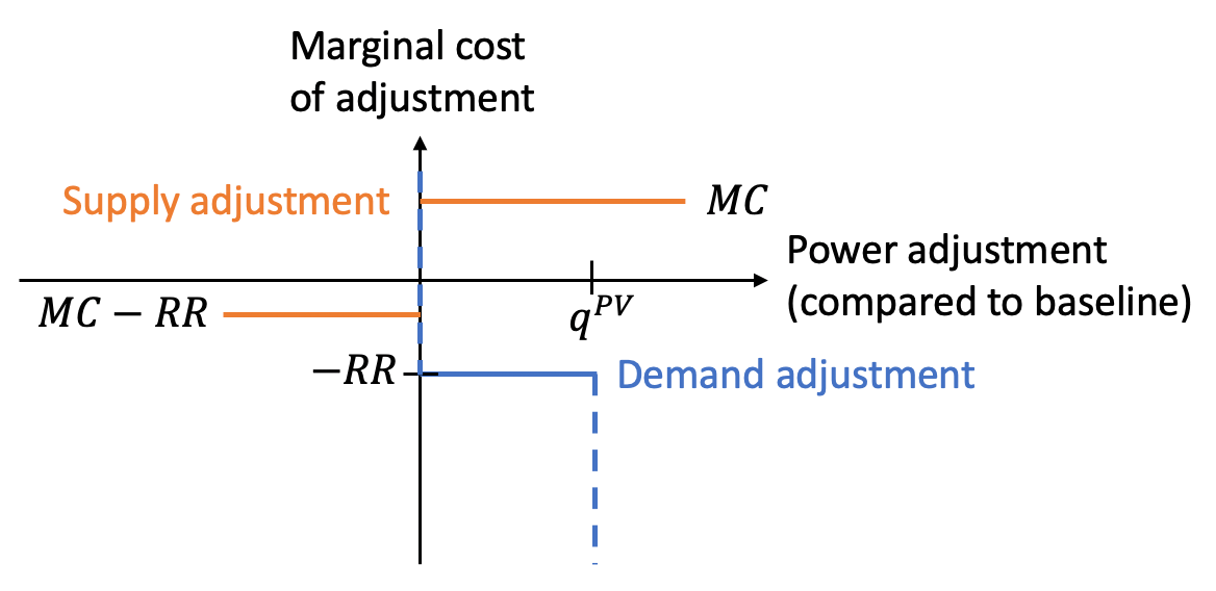
\includegraphics[height=3.2cm]{Market_power_normal_3.png}
    \caption{Market under normal supply conditions}
    \label{fig:lem_adjustment_normal}
  \end{subfigure}\hspace{0.5cm}
  \begin{subfigure}[t]{.485\linewidth}
    \centering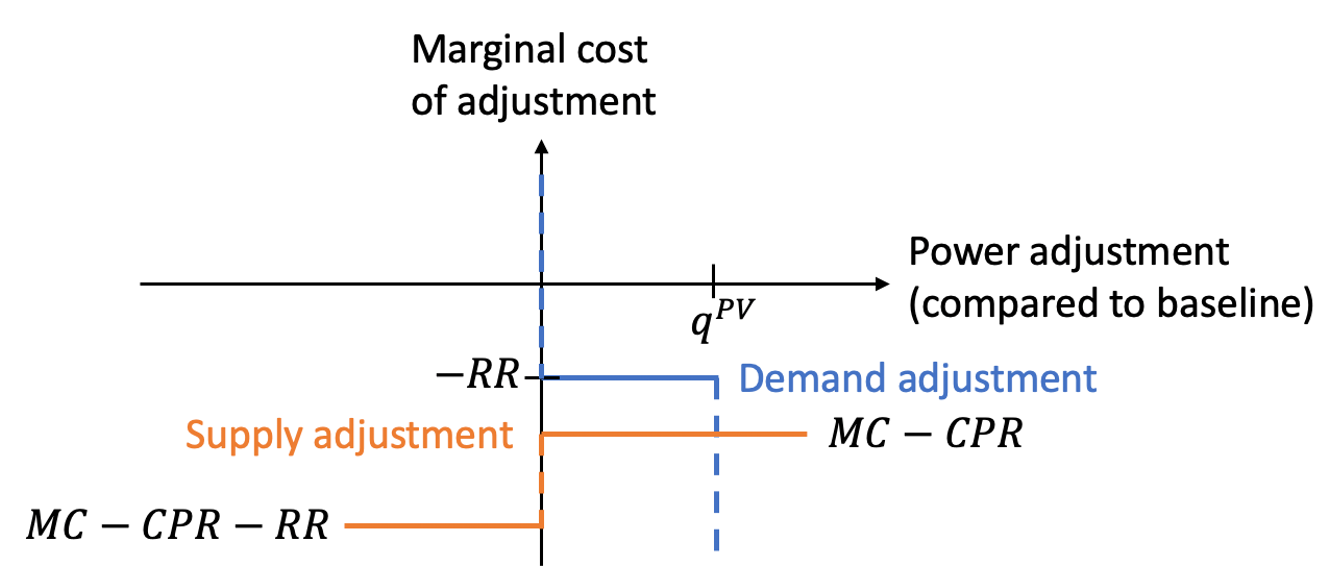
\includegraphics[height=3.2cm]{Market_power_adjustment_3.png}
    \caption{Market under requirement to increase net load} 
    \label{fig:lem_adjustment}
  \end{subfigure}
\caption{Market for power adjustment (compared to baseline)}
\end{figure}

We further analyze the bidding behavior of HCE. HCE is a cooperative and follows a complex combination of objectives, including commitments to resilience and energy supply sustainability. To derive the optimal bidding strategy, we abstract from that complexity and model HCE as a profit-maximizing entity, as many of those objectives are incorporated in their long-term investment and procurement decisions. Furthermore, with our focus on PV, this essentially translates into a cost-minimization problem. The decision variable is HCE's bidding strategy through which they can influence demand and supply participating in the TS,

\begin{align}
    \max \pi_\mathbf{b} &= \sum_t [\sum_{ij} (q^d_{ijt}(\mathbf{b}) -  q^s_{ijt}(\mathbf{b})) RR - MC_t q^{WS}_t + peak_t CPR_t |q^{WS}_t - \overline{q}^{WS}_t| ] + T(\mathbf{b}) \nonumber \\
    & s.t. \sum_{ij} q^d_{ijt}(\mathbf{b}) =  \sum_{ij} q^s_{ijt}(\mathbf{b}) + q^{WS}_t
\end{align}

The objective function includes income from net retail sales and the cost of energy procurement. The latter depend on the occurrence of a peak event, with $peak_t \in \{0;1\}$. Finally, the objective function includes the income of operating the transactive system. 

Under normal conditions ($peak_t = 0$), of course, HCE would not be willing to pay a customer the retail rate to reduce generation. Instead, it would sell additional generation at its long-term marginal supply cost $MC_t$ (and even take a price less than the fixed retail rate). On the other hand, it would be only willing to reduce supply from the baseline scenario if paid the foregone profit, i.e. the difference between the retail rate and the marginal cost. The bids provided by HCE and consumers are illustrated in \cref{fig:lem_adjustment_normal}. The curves do not intersect and the market allocation is empty.

A situation is possible, however, during which HCE would want to decrease generation within its distribution grid or, equivalently, increase net load to a level of $\overline{q}^{WS}_t$. Such a peak event ($peak_t = 1$) could arise when there is an abundance of renewable energy in the grid. Then, the entity operating the overlying grid could be willing to pay a critical peak rate $CPR$ to HCE for net load increases. Alternatively, HCE would need to curtail renewable energy within its system and pay them a compensation of $CPR$. In that case, the HCE bid changes and it would be willing to sell at a negative price, $MC_t - CPR$, i.e. pay consumers to consume more. Further decreasing supplies would be even more costly for the marginal unit, as HCE would miss out on sales at the fixed retail rate. 
The bids provided by HCE and consumers are illustrated in \cref{fig:lem_adjustment}. Now, supply and demand adjustments intersect at a quantity of $q^{PV}_t$ and the clearing price $p_t$ would be determined between $p \in [MC_t - CPR, -RR]$. Because the price is negative, the cash flow reverses and buyers get paid, while the seller pays.

Importantly, given the outside options of customers (in particular net metering), our design of the TS does not trade energy or power, but rather the deviation from this baseline generation or consumption. Thus the clearing price on the market reflects the price of \textbf{deviating} from the baseline. As a result, bids must reflect the quantity by which customers would be willing to deviate from the baseline and at what price. 

\cref{fig:pv_profile} illustrates the resulting implementation of the market result for a single customer with a solar system. For demonstration purposes, solar generation is approximated as a continuous normal distribution function. Generation starts in the early morning hours, reaches its maximum around noon, and terminates after sunset. The home hub, on behalf of the controller, continuously provides bids for increasing net load/reducing generation at the respective current generation $q^{PV}$, according to the described bidding strategy. Now assume that an adverse event occurs at 1pm, the market is cleared, and the solar system is shut down. In that case, solar generation is reduced to zero. In the subsequent market interval, no current (counterfactual) generation is available. For the implementation at HCE that relies on deviation from a baseline, we therefore approximate the available load reduction (i.e. to keep the solar system curtailed) using the most recent measurement. Therefore, the reduction for which the customer is eventually paid at settlement, corresponds to the red straight line of counterfactual generation during the adverse event. Once the situation dissolves, the market does not clear anymore and the solar system goes back online.

\begin{figure}[t]
\centering
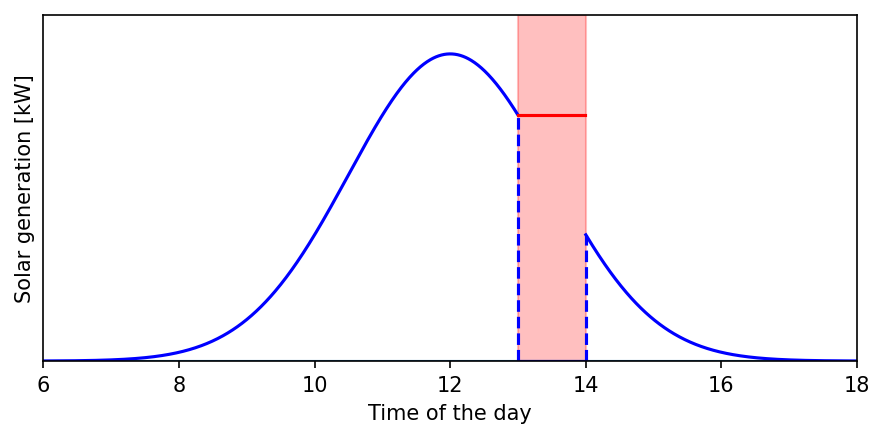
\includegraphics[scale=0.8]{TESS_PV_reduction.png}
\caption{PV curtailment}
\label{fig:pv_profile}
\end{figure}

TESS will integrate other DERs, specifically electric vehicle chargers and electric storage, at a later stage of the field deployment. Other device bidding functions will reflect the technical capabilities of each device and the opportunity costs and outside options of their owners. However, the baseline bidding strategies of PV panels as well as other DER come with significant challenges which will be discussed in \cref{sec:impl_challenges}.

\subsection{Settlement in TESS}\label{sec:hce_settlement}

In the last section, we described the bidding and market clearing in monetary terms, at given marginal costs and value. An additional problem in real-world systems, however, is that often actual costs/value only become clear in real-time or even  \textit{ex post}. One example is the cost of consuming or the value of producing during a coincident peak event. In the case of HCE, coincident  peak events happen at the time of the maximum net load in the Xcel system within a month. During the coincident peak, marginal consumption is significantly more expensive than during the rest of the month. However, it is unclear when it will actually happen within a month. For instance, overall load could be forecast to be very high during a day of the first week and the marginal supply costs would be supposedly very high, i.e. $MC_{coin} >> MC$. However, it might turn out that, later during the month, aggregate demand would be even higher. In that case, \textit{ex post}, the supply adjustment cost bid by HCE in the TS would have been wrong and any load adjustments would have been less valuable than previously thought. As a results, the bill credit required to be granted by HCE to responding customers would exceed the actual value they provided to the system.

Therefore, TESS will support tokens as a substitute for USD to bid in the TS. For a first implementation of our TS, we assume that customers have a prior of 1 token corresponding to the value of 1 USD. Therefore, any bids they make in USD could be translated into token bids on a 1:1 rate. 
At the end of the billing period, however, the market operator (here: HCE) would be able to calculate the total turnover of tokens during the month and determine the actual token value by comparing the turn-over to the savings achieved thanks to the operations of the TS. Multiplying the tokens collected by a customer with the final token value would give the final bill credit.

For the monthly bill of the customer, all tariffs need to be included again. The general electricity bill will be based on the read-out from the net meter, i.e. the net consumption during the billing period, multiplied by the fixed retail rate. In addition, TESS customers will be granted a bill credit, as foreseen in the DFP specification. Instead of a fixed amount per participating DER, the bill credit will depend on the turn-over of tokens the devices realized within TESS, multiplied by the value of a token. If, for instance, the solar panel of a customer disconnected due to an adverse event, the customer receives the product of the increase in net demand (equivalently, the reduction in generation) as compared to the base line, the token price paid by HCE for this deviation, and the token value in USD. As customers would not be willing to participate for a price below the fixed retail rate because of the net metering outside option, so their losses due to decreased solar generation will at least be off-set by the aggregate bill credit.

\subsection{Implementation Challenges}\label{sec:impl_challenges}

The implementation of TS in brownfield deployments comes with several challenges.
First, baseline approaches (i.e. providing demand flexibility as compared to a usual/expected load baseline) usually suffer from gaming. Customers could influence their baseline calculation to be able to report a bigger deviation from it and receive higher payments. In the case of PV, this risk is limited as HCE has access to the rated power of the system bidding as well as the PV measurements prior to the event. The latter can serve as a myopic forecast for the limited duration of a possible event requiring to increase net load. Moreover, HCE has access to data of solar panels that are not participating in TESS which provide a control baseline. Given these opportunities to validate customers' bids, we believe it is reasonable that customers bid their possible deviation to the best of their knowledge and specify the home hub to bid the latest measurement of PV generation as a possible deviation during the time when the system has not been curtailed. 
The problem becomes more severe, however, for other devices such as electric vehicles. It still needs to be determined how a baseline could be determined for other devices and whether information from such devices'  can be used to verify its bidding behavior.

Second, even if a baseline can be established, the baseline approach changes the distribution of surplus between the utility as well as customers with different devices. In the case of solar, customers will still enjoy the benefits of net-metering, even at times when the value of generation is far below the level of the fixed retail rate. Such effects can lead to inefficient investment in the long-term, as compared to a greenfield deployment with marginal value/cost bidding.

Third, the introduction of tokens opens up new opportunities, but also challenges. 
With regard to opportunities, tokens can be used to reimburse customers further for other beneficial actions, like the provision of data or energy efficiency investments. In theory, this compensation could be accomplished in USD, but other programs like Ohm Connect \citep{OhmConnect2020} and recent insights in gamification have shown that such tokens provide greater operational flexibility and might better be able to incentivize system-friendly behavior.
On the other hand, the introduction of tokens introduces another layer of uncertainty with regard to token value. Therefore, bidding should actually be based on the expected token value rather than on a fixed ``myopic'' assumption with respect to the value of a token.
In addition, some uncertainty remains regarding whether a token-based settlement mechanism might run afoul of government financial regulations, once the system is opened up for other stakeholders.

Finally, a TS alters the cash-flow of a utility. In non-TS, retail rates have been calculated to cover expected cost projections (as well as a risk premium), including increased costs during adverse events. The introduction of a TS provides the utility with more control capabilities and enables cost savings. The additional financial means -- i.e. the difference between the income from customer bills and the supply and operational costs -- should be able to cover the relevant bill credits. 
Established accounting model must be adjusted during a period of introducing a TS.

\subsection{Planned Extensions}\label{sec:extensions}

The current implementation of TESS at Basalt Vista in HCE territory represents a minimum viable product with PV and a double-sided centralized auction. In the following, we describe the planned extensions which we think will provide the most immediate value.

First, we are planning to incorporate electric vehicle charging as well as electric energy storage in Basalt Vista. 
Second, we plan to re-design bidding on behalf of HCE to reflect their planned participation in the Western balancing market. This will mean that they do not face distinct supply costs, depending on if the system operated under `normal' or `peak' conditions, rather costs that can change in real-time.
Third, we are planning to design an incentive-compatible settlement mechanism that ensures implementation of market results, even in an open TS.
Finally, we plan to extend TESS to support up to three distinct price discovery mechanisms simultaneously, i.e., energy prices (\$/MWh), storage prices (\$/MWh$^2$), and ramping prices (\$/MW) to address the challenges of dispatching resources when the marginal cost of supply is frequently zero.


\section{Conclusion and Future Work}\label{sec:conclusion}

Residential distribution systems are a potential source of system flexibility. This potential can be realized by an approach called transactive systems (TS) that coordinates residential devices through a market-based mechanism using price-based dispatch.
In this work, we present TESS, a open-source platform to develop, deploy, and operate TS in electric retail environments. TESS enables the dispatch of devices according to their physical state, customer preferences, and local and time-specific supply cost. 
Existing systems have been designed as closed control system. In contrast, we envision TESS to be a starting point for an open smart grid platform: the modularized structure will be able to incorporate multiple DER, enable third party access such as competing load aggregators, and provide the utility with the means for efficient and resilient operations of a system with increasing shares of variable renewable energy.

Furthermore, we describe TESS as we have specified it for a field implementation within the service territory of Holy Cross Energy in Colorado.
Previous implementations of TS have worked with experimental tariffs or side-payments to ensure participation and we identify such an approach as an existing hurdle to wide-scale deployment of TS. 
Instead, explicitly incorporating existing conditions such as a (non-transactive) tariff system can remove regulatory hurdles, build up trust with customers and utilities, and gain operational experience for the improvement of the system. 
In our field deployment, we designed our bidding approach to consider explicitly the economic incentives with regard to existing fixed retail rates and net-metering, and proposed the coordination of DER by TESS as an alternative design of the existing Distribution Flexibility Program (DFP), with bill credits being determined through the TS. 
We also explore the use of tokens to take into account the fact that, in today's system of long-term procurement contracts, the marginal cost of supply sometimes only becomes clear \textit{ex post}.
While these modifications might come at efficiency loss in the beginning, we hope that the gain in acceptance and experience will outweigh its costs in the long-run.

Future work should support the further modularization of TESS as well as designing modules. This includes, for instance, the design of new bidding functions, forecasting capabilities, market clearing, and billing processes.
Furthermore, more work should be invested in identifying the challenges of brownfield deployment and conceptualizing how TS can be adjusted to transition from an additional control component for DER to full-scale adoption, replacing existing tariff systems.


\pagebreak

%%%%%%%%%%%%%References%%%%%%%%%%%%%
\singlespacing
\newpage
\bibliographystyle{aea}
\bibliography{reference}
\clearpage


\funding{SLAC National Accelerator Laboratory is operated by Stanford University for the US Department of Energy under Contract DE-AC02-76SF00515. This work was funded under a grant from the US Department of Energy's Office of Electricity and completed in a collaboration with Holy Cross Energy Electric Cooperative in Glenwood Springs, Colorado and PostRoad Foundation in Oakland, California.}

\conflictsofinterest{The authors declare no conflict of interest.} 

\end{document}

